\documentclass[../../../main.tex]{subfiles}
\begin{document}



%\subsection{Mesh-gen: Python package modules and their integration}

All the algorithms developed during this work have been included in a Python package called \textit{mesh-gen}. 
Any reader interested in its use and operation can access it to complete all the concepts explained in the methodology of this work. 
In addition, the algorithms used to perform the matrix calculation of reticular structures and their optimisation have been published in another module, Spyffness. 
The main package consists of two main modules and a third module for generating the G-code that allows the generated structure to be printed in a non-planar form. 
This third module has not been integrated into the overall flow, in case the user is not interested in printing the structure this way. 
The names of the files will not be mentioned, as the package developed will continue to be maintained and evolved after the completion of this doctoral thesis, and some names may change. 

Before the modules are executed, a script is executed to check that all the necessary configuration for the correct execution of the package is defined. 
The logger is initialised and the execution folders are created, where all the files generated during execution will be saved: logs, graph and STL file.
Next, it checks whether there is a graph stored in the temporary folder. 
If so, the first module is not executed, and the graph stored in the temporary folder is used to generate the STL file. 
This was implemented to avoid duplicate executions and thus speed up overall execution. 
If there is no graph stored in the temporary folder, the geometry entered is processed, the points and sections of interest are extracted, and the first module is executed

The first module is responsible for generating the skeleton of the structure. 
This module receives as input the points and sections of the geometry to be processed and the values defined as the minimum allowed angle and pore size.
Next, all the routines that carry out the procedures explained in the methodology are executed. 
After obtaining the skeleton of the structure, it is saved in a pickle file as a Networkx object both in the folder created for execution and in the temporary folder, and the second module is executed.

The second module is responsible for generating the mesh of the generated structure. 
Within the configuration file, the user can choose whether or not to generate a fused mesh. 
If so, this module executes George W. Hart's modified algorithm and generates a mesh that is saved as an STL file. 
If not, a mesh will be generated based on the positioning of cylinders on the edges, which will not be joined, but is valid for printing the structure in 3D.
\cref{fig:workflow} shows a diagram of the overall flow of the main modules. To avoid redundancy of images, a flow for the case in which a merged mesh is not generated is not included, as the other case shown is more complete. This case would only include a step for generating the cylinders and another for exporting the STL file. The thickness of the cylinders or edges used in both cases is the same.

\begin{figure}[!htbp]
    \centering
    \includegraphics[width= 0.8\textwidth]{imgs/workflow.pdf}
    \caption{Overall workflow of the main modules of the mesh-gen package.}
    \label{fig:workflow}
\end{figure}

\subsection{Analysis of design parameters: minimum angle}

Although the objective of the developed algorithm is to generate self-supporting stochastic structures, the minimum angle that the edges can have was left as a design parameter so that it can be customised. 
While it is true that a 45$^\circ$ angle is sufficient to ensure self-sustainability, it is not necessarily the minimum angle that can be printed. 
Surfaces with smaller angles can also be printed under certain conditions. 
For example, if the printing speed is reduced and cooling is increased, it is possible to print with smaller angles. 
The minimum possible angle will always depend on the 3D printer and the printing conditions.
\cref{fig:angles} shows the angle distribution obtained for four different minimum angle values. 
It can be seen that there are effectively no edges with angles smaller than those established. 
In addition, the minimum angle is not the most common, but rather that it is usually approximately 5$^\circ$ greater than the minimum. 
There are very vertical angles that are usually present on the edges of the surface or on the last layer.  
This figure proves that the algorithm is capable of generating structures that ensure the self-sustainability of all edges.

\begin{figure}[!htbp]
    \centering
    \includegraphics[width= 0.6\textwidth]{imgs/angles.pdf}
    \caption{Distribution of angles obtained for four structures with different minimum allowed angle values.}
    \label{fig:angles}
\end{figure}

\subsection{Analysis of design parameters: pore area}

Another objective of the algorithm is to control the pore size in the generated structures. The definition of a pore is very ambiguous in reticular structures. 
It is difficult to define the physical limits that delimit the pore region. 
Closed-cell porous structures have a surface that partially or surrounds the pore, making it easy to define this region.
However, in reticular structures, no surface can give an idea of the limits of this region. 
In regular reticular structures, the pore can be defined as the volume of the unit cell used to design the structure.
However, in the case of stochastic structures, there is no repeating unit cell from which to deduce porosity. 
In these cases, it is more common to define the structure by its relative porosity rather than its pore size.
However, relative porosity cannot be known a priori because, in this case, it depends on the size of the edges that will be used later. 
Therefore, it was decided to discard the use of the term \textit{pore size} or \textit{pore volume} and use \textit{pore area} instead. 

The pore area was defined as the average area of the polygons that make up any section of the structure. 
Therefore, assuming that the volume to be processed has a constant section, if the number of polygons in each layer is the same, the average area must also be the same. 
For this reason, in the first iteration of the algorithm, the lower section of the volume is extracted, and the necessary triangles are generated in it so that the average size of the areas is that indicated by the pore area parameter. 
This process sets the number of polygons that will have to be in the following layers. 
If the processed volume did not have a constant section, the number of polygons to be generated is recalculated based on the variation in area. 
This ensures that the ratio of the perimeter to the number of polygons is constant. 
To calculate the pore area, the area of each of the polygons that make up each of the sections is calculated. 
Each of the polyhedra generated is stored in a dictionary where their points are classified according to whether they are base or apex points. 
The base points are then triangulated, the area of the triangle face is calculated, and the sum of all the areas is obtained.
As the triangulations are performed using the projections of each of the points, the value of the areas obtained is the value of the area of the projection onto the horizontal plane of each of the triangles, see \cref{fig:aberration}. 
Therefore, to obtain the actual area, it is divided by the cosine of the minimum angle, as this will be the most common aberration value. 
So, to obtain the desired pore area value throughout the layers, the pore area parameter set must be multiplied by the cosine of the minimum angle. 

\begin{figure}[!htbp]
    \centering
    

\tikzset{every picture/.style={line width=0.75pt}} %set default line width to 0.75pt        

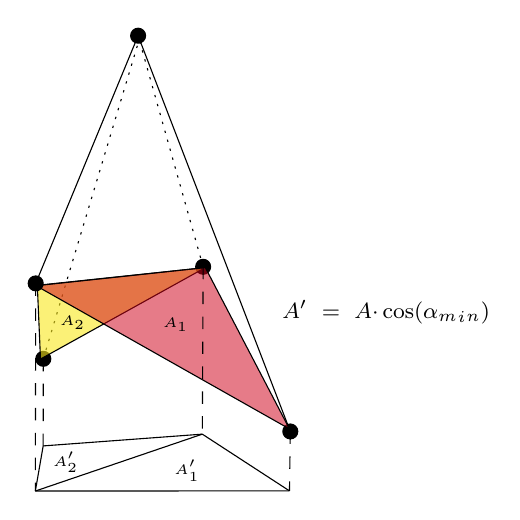
\begin{tikzpicture}[x=0.75pt,y=0.75pt,yscale=-1,xscale=1]
%uncomment if require: \path (0,300); %set diagram left start at 0, and has height of 300

%Shape: Circle [id:dp20203675621890882] 
\draw  [fill={rgb, 255:red, 0; green, 0; blue, 0 }  ,fill opacity=1 ] (75,183.4) .. controls (75,181.41) and (76.61,179.8) .. (78.6,179.8) .. controls (80.59,179.8) and (82.2,181.41) .. (82.2,183.4) .. controls (82.2,185.39) and (80.59,187) .. (78.6,187) .. controls (76.61,187) and (75,185.39) .. (75,183.4) -- cycle ;
%Shape: Circle [id:dp4460917567211786] 
\draw  [fill={rgb, 255:red, 0; green, 0; blue, 0 }  ,fill opacity=1 ] (152,139.07) .. controls (152,137.08) and (153.61,135.47) .. (155.6,135.47) .. controls (157.59,135.47) and (159.2,137.08) .. (159.2,139.07) .. controls (159.2,141.05) and (157.59,142.67) .. (155.6,142.67) .. controls (153.61,142.67) and (152,141.05) .. (152,139.07) -- cycle ;
%Shape: Circle [id:dp23372343609699975] 
\draw  [fill={rgb, 255:red, 0; green, 0; blue, 0 }  ,fill opacity=1 ] (194,218.4) .. controls (194,216.41) and (195.61,214.8) .. (197.6,214.8) .. controls (199.59,214.8) and (201.2,216.41) .. (201.2,218.4) .. controls (201.2,220.39) and (199.59,222) .. (197.6,222) .. controls (195.61,222) and (194,220.39) .. (194,218.4) -- cycle ;
%Shape: Circle [id:dp7435513334633294] 
\draw  [fill={rgb, 255:red, 0; green, 0; blue, 0 }  ,fill opacity=1 ] (120.67,27.73) .. controls (120.67,25.75) and (122.28,24.13) .. (124.27,24.13) .. controls (126.25,24.13) and (127.87,25.75) .. (127.87,27.73) .. controls (127.87,29.72) and (126.25,31.33) .. (124.27,31.33) .. controls (122.28,31.33) and (120.67,29.72) .. (120.67,27.73) -- cycle ;
%Straight Lines [id:da9245497792530712] 
\draw [color={rgb, 255:red, 0; green, 0; blue, 0 }  ,draw opacity=1 ] [dash pattern={on 0.84pt off 2.51pt}]  (78.6,183.4) -- (124.27,31.33) ;
%Straight Lines [id:da7005143254135355] 
\draw [color={rgb, 255:red, 0; green, 0; blue, 0 }  ,draw opacity=1 ] [dash pattern={on 0.84pt off 2.51pt}]  (155.6,139.07) -- (124.27,27.73) ;
%Straight Lines [id:da28064823401026573] 
\draw    (197.6,218.4) -- (124.27,27.73) ;
%Shape: Triangle [id:dp11918551614132744] 
\draw  [fill={rgb, 255:red, 248; green, 231; blue, 28 }  ,fill opacity=0.6 ] (77.24,183.52) -- (156.66,139.45) -- (75.71,148) -- cycle ;
%Shape: Triangle [id:dp7709931078112477] 
\draw  [fill={rgb, 255:red, 208; green, 2; blue, 27 }  ,fill opacity=0.52 ] (197.19,217.19) -- (75.12,148.19) -- (156.66,139.45) -- cycle ;
%Straight Lines [id:da7697818424224974] 
\draw [fill={rgb, 255:red, 0; green, 0; blue, 0 }  ,fill opacity=1 ]   (74.93,147.07) -- (124.27,27.73) ;
%Shape: Circle [id:dp25664476075983755] 
\draw  [fill={rgb, 255:red, 0; green, 0; blue, 0 }  ,fill opacity=1 ] (71.33,147.07) .. controls (71.33,145.08) and (72.95,143.47) .. (74.93,143.47) .. controls (76.92,143.47) and (78.53,145.08) .. (78.53,147.07) .. controls (78.53,149.05) and (76.92,150.67) .. (74.93,150.67) .. controls (72.95,150.67) and (71.33,149.05) .. (71.33,147.07) -- cycle ;
%Straight Lines [id:da5723635368812333] 
\draw  [dash pattern={on 4.5pt off 4.5pt}]  (74.93,147.07) -- (74.76,247.11) ;
%Straight Lines [id:da9477555281674963] 
\draw  [dash pattern={on 4.5pt off 4.5pt}]  (78.6,183.4) -- (78.53,225.37) ;
%Straight Lines [id:da7265146935260219] 
\draw  [dash pattern={on 4.5pt off 4.5pt}]  (155.6,139.07) -- (155.2,219.7) ;
%Straight Lines [id:da8482223625070795] 
\draw  [dash pattern={on 4.5pt off 4.5pt}]  (197.6,218.4) -- (197.2,247.03) ;
%Straight Lines [id:da135198346268814] 
\draw    (74.76,247.11) -- (197.2,247.03) ;
%Straight Lines [id:da7899881746363868] 
\draw    (155.2,219.7) -- (197.2,247.03) ;
%Straight Lines [id:da24200805108322687] 
\draw    (74.76,247.11) -- (155.2,219.7) ;
%Straight Lines [id:da38438776639593253] 
\draw    (78.53,225.37) -- (74.76,247.11) ;
%Straight Lines [id:da27704931617334616] 
\draw    (155.2,219.7) -- (78.53,225.37) ;

% Text Node
\draw (135,162.5) node [anchor=north west][inner sep=0.75pt]  [font=\tiny] [align=left] {$\displaystyle A_{1}$};
% Text Node
\draw (140.5,231) node [anchor=north west][inner sep=0.75pt]  [font=\tiny] [align=left] {$\displaystyle A'_{1}$};
% Text Node
\draw (82,227) node [anchor=north west][inner sep=0.75pt]  [font=\tiny] [align=left] {$\displaystyle A'_{2}$};
% Text Node
\draw (85.4,161.38) node [anchor=north west][inner sep=0.75pt]  [font=\tiny] [align=left] {$\displaystyle A_{2}$};
% Text Node
\draw (192.5,154) node [anchor=north west][inner sep=0.75pt]  [font=\footnotesize] [align=left] {$\displaystyle A'\ =\ A\cdotp \cos( \alpha _{m}{}_{i}{}_{n})$};


\end{tikzpicture}

    \caption{Illustration of the aberration suffered by triangles when projecting points onto the horizontal plane.}
    \label{fig:aberration}
\end{figure}


\cref{fig:areas} shows the evolution of the actual average angle compared to the configured angle for different values of the latter. 
It can be seen that the first layers have a lower area value due to this aberration. 
However, the area value then approximates the established value. In the last layers, the number of polygons may vary due to the termination criterion imposed. 
This is why the area varies in the last layers. In the cases of pore sizes of 15 and 20 $mm^2$, the actual area differs from the set value, probably because in these configurations the median angle differed from the angle to a greater degree than the minimum angle. 
Despite this, in the rest of the cases, it can be seen that the actual area value is the one set in most layers. 
The last case has so few layers that the area does not have time to settle before the end.
\cref{fig:areas_mean} shows the box plots for all areas present in each of the structures in \cref{fig:areas}.
Both figures confirm that pore area is a parameter that can be controlled by the algorithm. 
However, it is impossible to obtain a constant area value, as the same polygons are not used in each layer; instead, irregular tessellations are always used.

\begin{figure}[!htbp]
    \centering
    \includegraphics[width= 0.7\textwidth]{imgs/areas.pdf}
    \caption{Average value of the pore area in each layer for each pore area value set.}
    \label{fig:areas}
\end{figure}

\begin{figure}[!htbp]
    \centering
    \includegraphics[width= 0.7\textwidth]{imgs/areas_mean.pdf}
    \caption{Distribution of the area values in the whole structure for each pore area value set.}
    \label{fig:areas_mean}
\end{figure}

\subsection{Analysis of design parameters: edge length}

Although length is not a design parameter but rather a consequence of the design, it is interesting to analyse the edges that are generated. 
\cref{fig:lengths_edges} shows the total and layer-by-layer distribution of the length of the edges obtained in a structure created from a cylinder 20 \textit{mm} in diameter and 30 \textit{mm} high with a pore size of 10 $mm^2$.
It can be seen that the average size is similar in all layers, except in the last ones, where it increases. 
This may be due to the elongation of the edges of the previous layer, resulting from the established termination criterion. 
Although the distribution of lengths is indeed very wide, this was to be expected as it is a stochastic structure.

\begin{figure}[!htbp]
    \centering
    \includegraphics[width= 0.9\textwidth]{imgs/length.pdf}
    \caption{Left image: strut length distribution for a structure generated within a cylinder of 20 \textit{mm} diameter and 30 \textit{mm} height with a pore area of 10 $mm^2$. Right image: distribution of this length in each of the layers of the structure.}
    \label{fig:lengths_edges}
\end{figure}

\end{document}

